%%%%%%%%%%%%%%%%%%%%%%%%%%%%%%%%%%%%%%%%%%%%%%%%%%%%%%%%%%%%%
%% Begin exercise %%
%%%%%%%%%%%%%%%%%%%%%%%%%%%%%%%%%%%%%%%%%%%%%%%%%%%%%%%%%%%%%

\ex{Isolated DC-DC converters}

%%%%%%%%%%%%%%%%%%%%%%%%%%%%%%%%%%%%%%%%%%%%%%%%%%%%%%%%%%%%%
%% Task 1: Flyback converter %%
%%%%%%%%%%%%%%%%%%%%%%%%%%%%%%%%%%%%%%%%%%%%%%%%%%%%%%%%%%%%%
\task{Flyback converter}
A flyback converter with an input voltage range $U_\mathrm{1} = \SI{300}{\volt} \, \dots \, \SI{900}{\volt}$ is used to supply a control electronics unit. The converter delivers a rated output power of  $P_\mathrm{2} = \SI{30}{\watt}$ at a regulated (constant) output voltage of  $U_\mathrm{2} = \SI{15}{\volt}$. The flyback converter is operated in discontinuous conduction  mode with a constant frequency of  $f_\mathrm{s} = \SI{50}{\kilo\hertz}$. The turns ratio of the transformer is $N_\mathrm{1}/N_\mathrm{2}=60/12$, the magnetizing inductance on the primary side is $L_\mathrm{m} = \SI{760}{\micro\henry}$. The coupling between the primary and secondary windings is ideal and the converter operates in steady state.

%%%%%%%%%%%%%%%%%%%%%%%%%%%%%%%%%%%%%%%%%%%%%%%%%%%%%%%%%%%%%%%%%%%%%%%
 % Flyback converter Schematic
%%%%%%%%%%%%%%%%%%%%%%%%%%%%%%%%%%%%%%%%%%%%%%%%%%%%%%%%%%%%%%%%%%%%%%%
           
           \begin{figure}[htb]
                \begin{center}
                    \begin{circuitikz}[european currents,european resistors,american inductors]
                    \draw (0.5,0) to [short] ++(0.5,0)
                    to [diode, l=$D$]  ++(1.0,0)
                    to [short, -o, i=$i_2(t)$] ++(1.0,0)
                    to [open, o-o, v = $\hspace{2cm}u_2(t)$, voltage = straight] ++(0,-2) coordinate (A)
                    (-0.5,0) to [short, -o, i_<=$i_1(t)$] ++(-1.5,0)
                    to [open, o-o, v_= $u_1(t)\hspace{0.75cm}$, voltage = straight] ++(0,-3.75) coordinate (B)
                    (-0.5,0) to [inductor, n=l1] ++(0,-2) 
                    to [Tnpn, n=npn1, mirror] ++(0,-1.75) coordinate (C)
                    (0.5,0) to [inductor, n=l2, mirror] ++(0,-2) coordinate (D)
                    (D) to [short, -o] (A)
                    (C) to [short, -o] (B);
                    \draw let \p1 = (npn1.B) in node[anchor=south] at (\x1,\y1) {$T$};
                    \path (l1.ul dot) node[circ]{}
                        (l2.ur dot) node[circ]{};
                    \draw (l1.midtap) node[left]{$N_1$}
                    (l2.midtap) node[right]{$N_2$};
                    \draw[double, double distance=3pt, thick] let \p1=(l1.core west), \p2=(l2.core east) in (\x1/2+\x2/2, \y1) -- (\x1/2+\x2/2, \y2);
                \end{circuitikz}
            \end{center}
                \caption{Flyback converter topology}
                \label{fig:flyback_converter_topology}
            \end{figure}
        

\begin{table}[ht]
    \centering  % Zentriert die Tabelle
    \begin{tabular}{llll}
        \toprule
        
        Input voltage: &  $U_{\mathrm{1}} = \SI{300}{\volt} \, \dots \, \SI{900}{\volt}$ & Output voltage: & $U_{\mathrm{2}} = \SI{15}{\volt}$ \\ 
        Output power: & $P_2 = \SI{30}{\watt}$  & Transformation ratio: & $N_\mathrm{1}/N_\mathrm{2}=60/12$ \\ 
        Magn. inductance: & $L_\mathrm{m} = \SI{760}{\micro\henry}$ & Switching frequency: & $f_{\mathrm{s}} = \SI{50}{\kilo\hertz}$ \\ 
        \bottomrule
    \end{tabular}
    \caption{Parameters of the flyback converter.}  % Beschriftung der Tabelle
    \label{table:ex04_Parameters of the circuit}
\end{table}

\subtask{The input voltage is $U_\mathrm{1}=\SI{760}{\volt}$ at rated power at the output. What is the peak value $\hat i_\mathrm{1}$ of the primary current $i_\mathrm{1}$? What is the peak value $\hat i_\mathrm{2}$ of the secondary current $i_\mathrm{2}$? Calculate the duty cycle of the transistor for this operating point.} 

\begin{solutionblock}s
To determine the peak current  $\hat i_\mathrm{1}$ we consider the average power transfer
\begin{equation}
    P_\mathrm{2} = W_\mathrm{L} f_\mathrm{s}, \label{eq:output power ex04}
\end{equation}
with the stored magnetic energy
\begin{equation}
    W_\mathrm{L} = \frac{1}{2}L_\mathrm{m}\hat i_\mathrm{1}^2. \label{eq:energy primary inductance ex04}
\end{equation}
Insertig delivers
\begin{equation}
    P_\mathrm{2} = \frac{1}{2}L_\mathrm{1}\hat i_\mathrm{1}^2 f_\mathrm{s}.\label{eq:output power with IDach ex04}
\end{equation}
Solving for $\hat i_\mathrm{1}$ yields the peak current
\begin{equation}
    \hat i_\mathrm{1} = \sqrt{\frac{2P_\mathrm{2}}{L_\mathrm{m}f_\mathrm{s}}}= \sqrt{\frac{2\cdot\SI{30}{\watt}}{\SI{760}{\micro\henry}\cdot\SI{50}{\kilo\hertz}}}=\SI{1.257}{\ampere}.
\end{equation}
Since an in ideal transformer is assumed, the secondary peak current directly follows from the primary peak current and the turns ratio:
\begin{equation}
    \hat i_\mathrm{2} = \hat i_\mathrm{1} \frac{N_\mathrm{1}}{N_\mathrm{2}} = \SI{1.257}{\ampere} \cdot \frac{60}{12} = \SI{6.28}{\ampere}.
\end{equation}
Because of DCM the the voltage transfer ratio is
\begin{equation}
    \frac{U_2}{U_1} = \frac{D^2}{2} \frac{\Delta i_\mathrm{m,max}}{\overline{i}_2}. \label{eq:Duty cycle ex04}
\end{equation}
The yet unknown current ripple can be determined via the switch-on interval
\begin{equation}
    \Delta i_\mathrm{m,max}= \frac{T_\mathrm{s} \cdot U_1}{L_\mathrm{m}} = \frac{\frac{1}{\SI{50}{\kilo\hertz}}\cdot \SI{760}{\volt}}{\SI{760}{\micro\henry}}=\SI{20}{\ampere}.
\end{equation}
Inserting in \eqref{eq:Duty cycle ex04} and solving for D yields:

\begin{equation}
    D = \sqrt{\frac{2U_2\overline{i}_2}{U_1\Delta i_\mathrm{m,max}}} = \sqrt{\frac{2\cdot \SI{15}{\volt}\cdot\SI{30}{\watt}}{\SI{760}{\volt}\cdot\SI{15}{\volt}\cdot\SI{20}{\ampere}}} = 0.063.
\end{equation}

\end{solutionblock}

\subtask{The input voltage is  $U_\mathrm{1}=\SI{382}{\volt}$ at nominal load. Calculate and sketch the following voltage and current curves for this operating case over one cycle period: $u_\mathrm{T}(t), u_\mathrm{s}(t), i_\mathrm{2}(t), i_\mathrm{1}(t)$. Here, $u_\mathrm{T}(t)$ is the transistor voltage and $u_\mathrm{s}(t)$ is the voltage on the secondary side of the transformer.}

\begin{solutionblock}
    Because of a different voltage value the duty cycle $D$ has changed:
    \begin{equation}
        \Delta i_\mathrm{m,max}= \frac{T_\mathrm{s} \cdot U_1}{L_\mathrm{m}} = \frac{\frac{1}{\SI{50}{\kilo\hertz}}\cdot \SI{382}{\volt}}{\SI{760}{\micro\henry}}=\SI{10.05}{\ampere}.
    \end{equation}
    \begin{equation}
        D = \sqrt{\frac{2U_2\overline{i}_2}{U_1\Delta i_\mathrm{m,max}}} = \sqrt{\frac{2\cdot \SI{15}{\volt}\cdot\SI{30}{\watt}}{\SI{382}{\volt}\cdot\SI{15}{\volt}\cdot\SI{10.05}{\ampere}}} = 0.125.
    \end{equation}
    Trough this result $T_\mathrm{on}$ can be calculated as:
    \begin{equation}
        T_\mathrm{on} = D T_\mathrm{s} = 0.125 \cdot \frac{1}{\SI{50}{\kilo\hertz}} = \SI {2.5}{\micro\s}.
    \end{equation}
    The flyback converter in DCM has three different switch states $T_\mathrm{on}, T'_\mathrm{off}$ and $T''_\mathrm{off}$. Because of this $D'$ has be calculated as:
    \begin{equation}
        D' = \frac{N_\mathrm{2}U_\mathrm{1}}{N_\mathrm{1}U_\mathrm{2}}D = \frac{12\cdot \SI{382}{\volt}}{60 \cdot \SI{15}{\volt}} D = 0.637,
    \end{equation}
    \begin{equation}
        T'_\mathrm{off} = D' T_\mathrm{s} = 0.637 \cdot \frac{1}{\SI{50}{\kilo\hertz}} = \SI {12.7}{\micro\s},
    \end{equation}
    \begin{equation}
        T''_\mathrm{off}= T_\mathrm{s} -T_\mathrm{on}-T'_\mathrm{off} = \frac{1}{\SI{50}{\kilo\hertz}} - \SI {2.5}{\micro\s} - \SI {12.7}{\micro\s} = \SI {4.8}{\micro\s}.
    \end{equation}
    The intervals are determined. In the following the voltage values in the three intervals are calculated:
    The first interval is 0 < t < $T_\mathrm{on}$. In this interval the transistor conducts and therefore the voltage $U_\mathrm{T}=0$
    The following applies to the voltage on the secondary side:
    \begin{equation}
        u_\mathrm{T} = U_1 + \frac{N_1}{N_2}U_\mathrm{2}.\label{eq:voltageTransistorTask1 ex04}
    \end{equation}
    In this interval the $U_\mathrm{2} = u_\mathrm{s}$. As $u_\mathrm{T}=0$ = 0 follows:
    \begin{equation}
        u_\mathrm{s} = -U_1 \frac{N_2}{N_1} = -\SI{382}{\volt}\cdot\frac{12}{60} = \SI{-76.4}{\volt}.
    \end{equation}
    The second interval is $T_\mathrm{on}$ < t < $T'_\mathrm{off}$. In this interval the transistor blocks. For this calculaion \eqref{eq:voltageTransistorTask1 ex04} can be used again as:
    \begin{equation}
        u_\mathrm{T} = \SI{382}{\volt} + \frac{60}{12}\cdot\SI{15}{\volt} = \SI{457}{\volt}.
    \end{equation}
    Because of the conducting diode $U_\mathrm{2} = u_\mathrm{s} = \SI{15}{\volt}$.
    The third interval is $T_\mathrm{on}+T'_\mathrm{off}$ < t < $T_\mathrm{s}$. In this interval the diode is not conducting and der transistor blocks. From this follows $u_\mathrm{T} = U_1$ and $u_\mathrm{s}=0$
    Current $i_\mathrm{1}(t)$ can only be present when the transistor is switched on. When the transistor is switched on, the current value rises to the peak value $\hat i_\mathrm{1}= \SI{1.257}{\ampere}$. Current $i_\mathrm{2}(t)$ is the discharge current of the secondary winding when the diode is conducting. The discharge current starts at the peak value of the secondary side $\hat i_\mathrm{2}= \SI{6.28}{\ampere}$.
    \begin{solutionfigure}[htb]
    \centering
    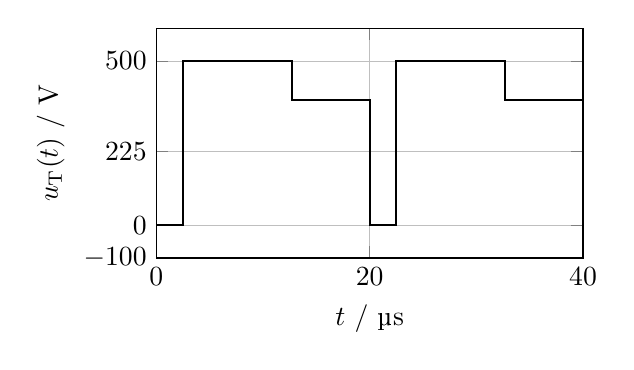
\begin{tikzpicture}
    \begin{axis}[
        width=7cm, height=4.5cm,
        grid=both,
        major grid style={line width=.2pt,draw=gray!50},
        minor grid style={line width=.1pt,draw=gray!20},
        xlabel={$t$ / µs},
        ylabel={$u_\mathrm{T}(t)$ / V},
       % title={$i_\mathrm{L}$ for minimum output power},
        xmin=0, xmax=40,
        ymin=-100, ymax=600,
        xtick={0, 20, 40},
        ytick={-100, 0, 225, 500},
        ]
        % Einschaltverhalten graph
        \addplot[
            thick,
            mark=none,
            color=black,
        ] coordinates {
            (0,0) (2.5,0) (2.5, 500) (12.7, 500) (12.7, 382) (20, 382) (20, 0) (22.5, 0)(22.5, 500) (32.7, 500) (32.7, 382) (40, 382)
        };
    \end{axis}
    \end{tikzpicture} 
    \hspace{1cm} % Abstand zwischen den beiden Diagrammen
    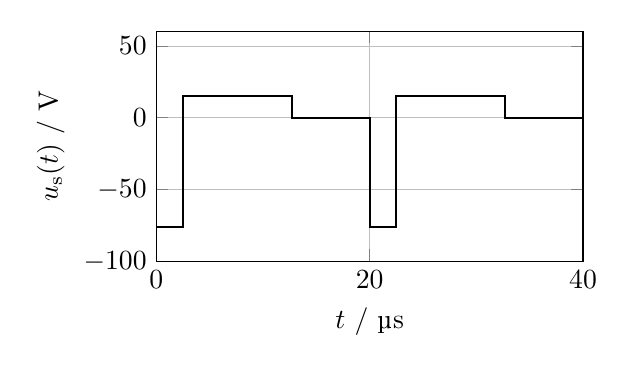
\begin{tikzpicture}
        \begin{axis}[
            width=7cm, height=4.5cm,
            grid=both,
            major grid style={line width=.2pt,draw=gray!50},
            minor grid style={line width=.1pt,draw=gray!20},
            xlabel={$t$ / µs},
            ylabel={$u_\mathrm{s}(t)$ / V},
           % title={$i_\mathrm{L}$ for minimum output power},
            xmin=0, xmax=40,
            ymin=-100, ymax=60,
            xtick={0, 20, 40},
            ytick={-100, -50, 0, 50},
            ]
            % Einschaltverhalten graph
            \addplot[
                thick,
                mark=none,
                color=black,
            ] coordinates {
                (0,0) (0,-76.4) (2.5,-76.4) (2.5, 15) (12.7, 15) (12.7, 0) (20, 0) (20, 0) (20, -76.4) (22.5, -76.4)(22.5, 15) (32.7, 15) (32.7, 0) (40, 0)
            };
        \end{axis}
        \end{tikzpicture} 
    \caption{Display of the voltage $u_\mathrm{T}(t)$ and $u_\mathrm{s}(t)$.}
    \label{fig:voltageTransistorPeriodTask1}

          
    \end{solutionfigure}
    \begin{solutionfigure}[htb]
    \centering
    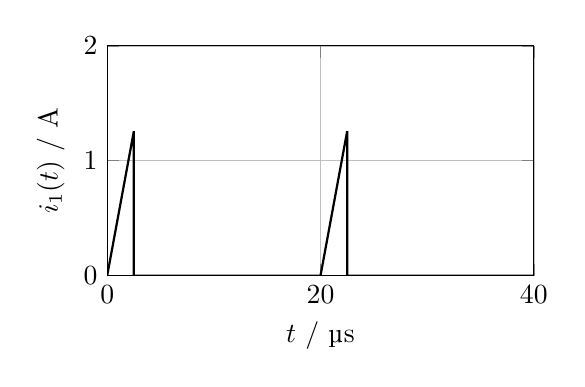
\begin{tikzpicture}
    \begin{axis}[
        width=7cm, height=4.5cm,
        grid=both,
        major grid style={line width=.2pt,draw=gray!50},
        minor grid style={line width=.1pt,draw=gray!20},
        xlabel={$t$ / µs},
        ylabel={$i_\mathrm{1}(t)$ / A},
       % title={$i_\mathrm{L}$ for minimum output power},
        xmin=0, xmax=40,
        ymin=-0, ymax=2,
        xtick={0, 20, 40},
        ytick={0, 1,2},
        ]
        % Einschaltverhalten graph
        \addplot[
            thick,
            mark=none,
            color=black,
        ] coordinates {
            (0,0) (2.5, 1.257) (2.5, 0) (20, 0)(22.5,  1.257) (22.5,  0) (40, 0)
        };
    \end{axis}
    \end{tikzpicture} 
    \hspace{1cm} % Abstand zwischen den beiden Diagrammen
    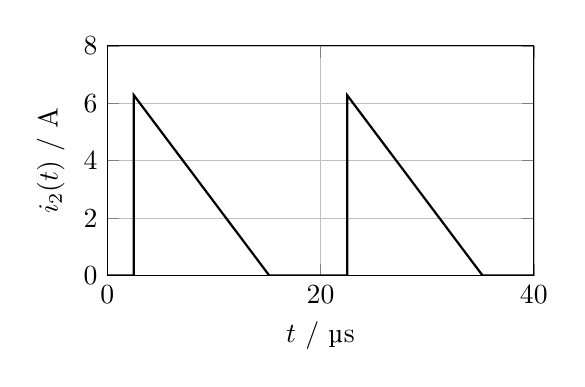
\begin{tikzpicture}
        \begin{axis}[
            width=7cm, height=4.5cm,
            grid=both,
            major grid style={line width=.2pt,draw=gray!50},
            minor grid style={line width=.1pt,draw=gray!20},
            xlabel={$t$ / µs},
            ylabel={$i_\mathrm{2}(t)$ / A},
           % title={$i_\mathrm{L}$ for minimum output power},
            xmin=0, xmax=40,
            ymin=-0, ymax=8,
            xtick={0, 20, 40},
            ytick={0, 2,4,6,8},
            ]
            % Einschaltverhalten graph
            \addplot[
                thick,
                mark=none,
                color=black,
            ] coordinates {
                (0,0) (2.5, 0) (2.5, 6.28) (15.2, 0) (22.5, 0)(22.5, 6.28) (35.2, 0) (40, 0)
            };
        \end{axis}
        \end{tikzpicture} 
    \caption{Display of the current $i_\mathrm{1}(t)$.}
    \label{fig:currentSecondarySideTask1}
    \end{solutionfigure}
\end{solutionblock}


\subtask{Determine the mean value $\overline i_\mathrm{T}$ and the RMS current $I_\mathrm{T}$ through the transistor. Also,  determine the mean value $\overline i_\mathrm{D}$ and the RMS current $I_\mathrm{D}$ through the diode. What is the maximum reverse voltage load $u_\mathrm{T, max}$ of the transistor and $u_\mathrm{D, max}$ of the diode? Consider the same operation conditions as in the previous subtask.}
\begin{solutionblock}
    The current is in the form of a triangle. Therefore, the average value must first be determined over the $T_\mathrm{on}$. This value corresponds to the area of the triangle. The value is divided by $T_\mathrm{S}$ to obtain the average value over the entire period. This gives:
    \begin{equation}
        \overline{i}_\mathrm{T} = \frac{1}{T_\mathrm{S}}\frac{1}{2}\hat i_\mathrm{1}T_\mathrm{on}=\frac{1}{\SI{20}{\micro\s}}\cdot\frac{1}{2}\cdot\SI{1.257}{\ampere}\cdot\SI{2.5}{\micro\s}=\SI{78.53}{\milli\ampere}.
    \end{equation}
    To determine the RMS value of the transistor current, the straight line equation of the applied current must be created and inserted, which leads to
    \begin{equation}
        I_\mathrm{T}^2=\frac{1}{T_\mathrm{S}} \int_{0}^{T_\mathrm{S}} i_\mathrm{1}^2(t) \,\mathrm{d}t \ = \frac{1}{T_\mathrm{S}}\int_{0}^{T_\mathrm{on}} \frac{\hat i_\mathrm{1}^2t^2}{T_\mathrm{on}^2} \,\mathrm{d}t \ =  \frac{\hat i_\mathrm{1}^2T_\mathrm{on}}{3T_\mathrm{on}},
    \end{equation}
    \begin{equation}
        I_\mathrm{T} = \hat i_\mathrm{1} \sqrt{\frac{T_\mathrm{on}}{3T_\mathrm{S}}}= \SI{1.257}{\ampere}\cdot\sqrt{\frac{\SI{2.5}{\micro\s}}{3\cdot\SI{20}{\micro\s}}}= \SI{256.58}{\milli\ampere}.
    \end{equation}
    The mean value for the current $i_\mathrm{D}$ and the RMS value for  $i_\mathrm{D}$ are determined as already explained:
    \begin{equation}
        \overline{i}_\mathrm{D} = \frac{1}{T_\mathrm{S}}\frac{1}{2}\hat i_\mathrm{2}T_\mathrm{off}=\frac{1}{\SI{20}{\micro\s}}\cdot\frac{1}{2}\cdot\SI{6.28}{\ampere}\cdot\SI{12.7}{\micro\s}=\SI{2}{\ampere},
    \end{equation}

    \begin{equation}
        I_\mathrm{D} = \hat i_\mathrm{2} \sqrt{\frac{T_\mathrm{off}}{3T_\mathrm{S}}}= \SI{6.28}{\ampere}\cdot\sqrt{\frac{\SI{12.7}{\micro\s}}{3\cdot\SI{20}{\micro\s}}}= \SI{2.89}{\ampere}.
    \end{equation}
    The voltage  $u_\mathrm{T,max}$ is calculated as in \eqref{eq:voltageTransistorTask1 ex04} as:
    \begin{equation}
        u_\mathrm{T,max} = U_\mathrm{1} + \frac{N_\mathrm{1}}{N_\mathrm{2}}U_\mathrm{2}= \SI{382}{\volt}+\frac{60}{12}\cdot\SI{15}{\volt}= \SI{457}{\volt}.
    \end{equation}
    \eqref{eq:voltageTransistorTask1 ex04} is used again, but now for the secondary side. This leads to:
    \begin{equation}
        u_\mathrm{D,max} = U_\mathrm{2} + \frac{N_\mathrm{2}}{N_\mathrm{1}}U_\mathrm{1}= \SI{15}{\volt}+\frac{12}{60}\cdot\SI{382}{\volt}= \SI{91.4}{\volt}.
    \end{equation}

\end{solutionblock}

\subtask{How much energy is transferred from the input to the output per switching period $\Delta E$ and what is the resulting average power $P$ (consider the same operation conditions as in the previous subtask)? What happens if there is no ideal voltage source on the output side but an unloaded capacitor and the circuit is operated with $D>0$?}

\begin{solutionblock}
    The energy on the primary side can be determined with \eqref{eq:energy primary inductance ex04}:
    \begin{equation}
        W_\mathrm{L} = \frac{1}{2}\cdot \SI{760}{\micro\henry} \cdot \SI{1.257}{\ampere} = \SI{600}{\micro\joule}.
    \end{equation}
    Since this is an ideal converter, no losses are assumed. 
    To determine the average power ${P}$, the transmitted energy must be divided by the period duration $T_\mathrm{s}$, as follows:
    \begin{equation}
        {P} = \frac{W_\mathrm{L}}{T_\mathrm{s}} = \frac{\SI{600}{\micro\joule}}{\SI{20}{\micro\s}}=\SI{30}{\watt}.
    \end{equation}
At each switching interval, energy is pushed into the capacitor, the voltage of which continues to rise until a component fails due to a lack of dielectric strength.    
\end{solutionblock}

%%%%%%%%%%%%%%%%%%%%%%%%%%%%%%%%%%%%%%%%%%%%%%%%%%%%%%%%%%%%%%%%%%%%%%%%%%%%%%%%%%%%%%%%%%%%%%%%%%%%%%%%%%
%% Task 2: Forward converter with asymmetric half-bridge
%%%%%%%%%%%%%%%%%%%%%%%%%%%%%%%%%%%%%%%%%%%%%%%%%%%%%%%%%%%%%%%%%%%%%%%%%%%%%%%%%%%%%%%%%%%%%%%%%%%%%%%%%%

\task{Forward converter with asymmetric half-bridge}

The schematic of a forward converter with an asymmetric half-bridge is shown in \autoref{fig:ex04_ForwardConverterWithAsymHalfBridge}. 
For the calculations the diodes and transistors are considered as ideal components.

%%%%%%%%%%%%%%%%%%%%%%%%%%%%%%%%%%%%%%%%%%%%%%%%%%%%%%%%%%%%%%%%%%%%%%%%%%
%  Forward converter with asymmetric half-bridge
%%%%%%%%%%%%%%%%%%%%%%%%%%%%%%%%%%%%%%%%%%%%%%%%%%%%%%%%%%%%%%%%%%%%%%%%%%

\begin{figure}[ht]
    \begin{center}
        \begin{circuitikz}[european currents,european resistors,american inductors]
            \draw 
                    % Base point for voltage supply
                    (0,0) coordinate (jU1v)
                    % Add supply U1
                    (jU1v) to [V=$U_1$] ++(0,-7.5) coordinate (jU1g)
                    % Add junction for Transistor TBc
                    (jU1v) to [short,-*] ++(2,0) coordinate (jTBc)
                    % Add junction for Transistor TBe
                    (jTBc) ++ (0,-2) coordinate (jTBe)
                    % Add transistor TB
                    % (jTBc) ++ (0,-1) [Tnpn, n=npn1](TB){}
                    (jTBc) ++ (0,-2) node[npn, anchor=E](TB){}
                    % At transistor label T2
                    (TB)  node[anchor=east,color=black]{$T_\mathrm{B}$}                     
                    % Connect Transistor
                    (jTBe) to [short,-] (TB.E)
                    (jTBc) to [short,-] (TB.C)
                    (TB.B) to [sqV] ++(-1,0);                    
                    % Add inductor transistor TB
                    %(jTBe) to [L,l=$L_\mathrm{T}$,n=L1,v_<=$U_\text{s}$, voltage shift=0.5, voltage=straight] (jTBc);
            \draw                    
                    % Add connection point of the diode DFP
                    (jTBe) ++(0,-3) coordinate (jDFPa)
                    % Add diode DFP
                    (jDFPa) to [D,l^=$D_\mathrm{Fp}$] (jTBe)
                    % Add connection to U1g
                    (jDFPa) to [short,-] (jU1g)
                    % Add junction for transformer Ltpv
                    (jTBc) to [short,-] ++(2,0)  coordinate  (jLtpv)
                    % Add arrow and Text
                    (jTBc) ++(1,0) node[currarrow](IP){}  
                    (IP)  node[anchor=south,color=black]{$i_\mathrm{p}$}                   
                    % Add junction for Transistor
                    (jLtpv) ++(0,-3) coordinate (jTd)
                    % Add junction for Transistor
                    (jTd) ++(0,-3) coordinate (jTs)
                    % Add transistor T2
                    (jTs) ++ (0,1.5) node[nigfete,xscale=-1](Trans1){}
                    % At transistor label T2
                    (Trans1)  node[anchor=east,color=black]{$T$}                     
                    % Connect Transistor
                    (jTs) to [short,-] (Trans1.S)
                    (jTd) to [short,-] (Trans1.D)
                    (Trans1.G) to [sqV] ++(1,0)
                    % Add connection to diode DFp
                    (jTs) to [short,-*] (jDFPa)
                    % Assign Transistor drain junction to primary junction point
                    (jTd) coordinate  (jLtpg)
                    % Add transformer primary inductor with voltage arrow
                    (jLtpv) to [L, n=Ltp, v_=$U_\text{p}$, voltage=straight] ++(0,-3) coordinate (jLtpg)
                    % Add junctions for secondary inductor
                    (jLtpv) ++(0.8,0) coordinate  (jLtsv) 
                    (jLtpg) ++(0.8,-0.5) coordinate  (jLtsgx)
                    % Add winding text
                    (jLtpg) node[left] {$N_\mathrm{p}$};         
                    % Add iron core
            \draw 
                    (jLtpv) ++(0.5,-0.5) coordinate  (jLtcorev) 
                    (jLtpg) ++(0.5,0.5) coordinate  (jLtcoreg)
                    (jLtcorev) to [short, double, double distance=3pt, thick]  (jLtcoreg)
                    let \p1 = (jLtcorev), \p2 = (jLtcoreg) in [double, double distance=3pt, thick]
                    (\x1/2+\x2/2, \y1) -- (\x1/2+\x2/2, \y2); 
            \draw 
                    % Add transformer secondary inductor with voltage arrow
                    (jLtsv) to [L,n=Lts,v^=$U_\text{s}$, voltage shift=0.5, voltage=straight] ++(0,-3) coordinate (jLtsg)
                    % Add winding text
                    (jLtsg) node[right] {$N_\mathrm{s}$};     
                    \path (Ltp.ul dot) node[circ]{};
                    \path (Lts.ul dot) node[circ]{};                    
            \draw
                    % Add arrow and Text
                    (jLtsv) ++(0.5,0) node[currarrow](IS){}  
                    (IS)  node[anchor=south,color=black]{$i_\mathrm{s}$}
                     % Add D1
                    (jLtsv) to  [D,l^=$D_1$] ++ (2,0) coordinate (jD1k)
                    % Add junction point for DFsk
                    (jD1k)  to [short,-*] ++(0,0) coordinate (jDFsk)
                    % Add junction point for DFsa
                    (jDFsk)  ++ (0,-3.5) coordinate (jDFsa)
                    % Add diode DFs
                    (jDFsa) to  [D,l^=$D_\mathrm{Fs}$]  (jDFsk)                    
                    % Add inductor L
                    (jDFsk) to [L,l=$L$,n=L1] ++(3,0) coordinate (jU2v)
                    % Add arrow and Text
                    (jDFsk) ++(0.5,0) node[currarrow](IL){}  
                    (IL)  node[anchor=south,color=black]{$i_\mathrm{L}$}
                    % Add output voltage U2
                    (jU2v) to [V=$U_2$] ++(0,-3.5) coordinate (jU2g)
                    % Add connection to DFs
                    (jU2g) to [short,-*] (jDFsa)
                    % Add connection to LTsgx
                    (jDFsa) to [short,-] (jLtsgx)
                    % Add connection to LTsgx
                    (jLtsgx) to [short,-] (jLtsg);

                \end{circuitikz}
    \end{center}
    \caption{Forward converter with asymmetric half-bridge.}
    \label{fig:ex04_ForwardConverterWithAsymHalfBridge}
\end{figure}


The parameters are listed in \autoref{fig:ex04_ForwardConverterWithAsymHalfBridge}.

%%%%%%%%%%%%%%%%%%%%%%%%%%%%%%%%%%%%%%%%%%%%%%%%%%%%%%%%%%%%%%%%%%%%%%%%%%
%  Parameter of the forward converter with asymmetric half-bridge
%%%%%%%%%%%%%%%%%%%%%%%%%%%%%%%%%%%%%%%%%%%%%%%%%%%%%%%%%%%%%%%%%%%%%%%%%%

\begin{table}[htb]
    \centering  % Zentriert die Tabelle
    \begin{tabular}{llll}
        \toprule
        Input voltage: &  $U_{\mathrm{1}} = \SI{325}{\volt}$ & Output voltage: & $U_{\mathrm{2}} = \SI{15}{\volt}$ \\ 
        Output power: & $P_{\mathrm{2}} = \SI{50}{\watt}$ & Switching frequency: & $f_{\mathrm{s}} = \SI{50}{\kilo\hertz}$ \\
        Turns ration: &  $N_{\mathrm{1}}/N_{\mathrm{2}}=10$ & Magnetizing inductance: & $L_{\mathrm{m}}=\SI{2}{\milli\henry}$  \\
        \bottomrule
    \end{tabular}
    \caption{Parameter overview of the circuit.}
    \label{table:Ex04_Forward converter with asymmetric half-bridge}
\end{table}
\FloatBarrier
The leakage inductance, the resistive losses, and the core losses of the transformer are negligible. 
The converter operates in steady-state conditions. Both transistors are controlled by the same signal.

\subtask{At what duty cycle $D$ does the circuit operate?}
\subtask{Calculate the average currents $\overline{i}_\mathrm{2}$ and $\overline{i}_\mathrm{1}$ over a switching cycle assuming ideal filtering of $i_\mathrm{2}$.}
\subtask{Calculate the peak value $\hat{i}_\mathrm{m}$ of the magnetizing current $i_\mathrm{m}$.}
\subtask{Sketch the signals $u_\mathrm{p}$, $i_\mathrm{m}$, $i_\mathrm{p}$ and $i_\mathrm{1}$ 
         considering the switching-induced ripples.}
\subtask{Calculate the minimal necessary input voltage $U_\mathrm{1}$, if $U_\mathrm{2}$ = \SI{20}{\volt} shall being constant.}
\subtask{Determine $L$ such that the ripple current $\Delta i_\mathrm{2}$ is $\SI{10}{\percent}$ of the 
         average output current $\overline{i}_\mathrm{2}$.}



%%%%%%%%%%%%%%%%%%%%%%%%%%%%%%%%%%%%%%%%%%%%%%%%%%%%%%%%%%%%%%%%%%%%%%%%%%%%%%%%%%%%%%%%%%%%%%%%%%%%%%%%%%
%% Task 3: Singled-ended forward converter (demagnetization winding)
%%%%%%%%%%%%%%%%%%%%%%%%%%%%%%%%%%%%%%%%%%%%%%%%%%%%%%%%%%%%%%%%%%%%%%%%%%%%%%%%%%%%%%%%%%%%%%%%%%%%%%%%%%

\task{Singled-ended forward converter (demagnetization winding)}

The power supply of a data processing system shall be realized by a singled-ended forward converter.


%%%%%%%%%%%%%%%%%%%%%%%%%%%%%%%%%%%%%%%%%%%%%%%%%%%%%%%%%%%%%%%%%%%%%%%%%%
%  Single Ended Forward Converter
%%%%%%%%%%%%%%%%%%%%%%%%%%%%%%%%%%%%%%%%%%%%%%%%%%%%%%%%%%%%%%%%%%%%%%%%%%

\begin{figure}[ht]
    \begin{center}
        \begin{circuitikz}[european currents,european resistors,american inductors]
            \draw 
                    % Base point for voltage supply
                    (0,0) coordinate (jU1v)
                    % Add supply U1
                    (jU1v) to [V=$U_\mathrm{1}$] ++(0,-4) coordinate (jU1g)
                     % Add junction for inductor LT
                    (jU1v) to [short,-*] ++(2,0) coordinate (jLTv)
                    % Add junction for diode D3
                    (jLTv) ++ (0,-2) coordinate (jD3k)
                    % Add inductor LTv
                    (jD3k) to [L,l=$N_\mathrm{3}$,n=L1,v_<=$U_\mathrm{3}$, voltage shift=0.5, voltage=straight] (jLTv);
                    \path (L1.ul dot) node[circ]{};
            \draw                    
                    % Add arrow and Text
                    (jD3k) ++(0,-0.5) node[currarrow,rotate=90](IT){}  
                    (IT)  node[anchor=east,color=black]{$i_\mathrm{3}$}
                    % Add connection point of the diode D3
                    (jD3k) ++(0,-2) coordinate (jD3a)
                    % Add diode D3
                    (jD3a) to [D,l^=$D_\mathrm{3}$] (jD3k)
                    % Add connection to U1g
                    (jD3a) to [short,-] (jU1g)
                    % Add junction for transformer Ltpv
                    (jLTv) to [short,-] ++(2.5,0)  coordinate  (jLtpv)
                    % Add arrow and Text
                    (jLTv) ++(1,0) node[currarrow](IP){}  
                    (IP)  node[anchor=south,color=black]{$i_\mathrm{p}$}                   
                    % Add junction for Transistor
                    (jLtpv) ++(0,-2) coordinate (jTd)
                    % Add junction for Transistor
                    (jTd) ++(0,-2) coordinate (jTs)
                    % Add transistor T2
                    (jTs) ++ (0,1) node[nigfete,xscale=-1](Trans1){}
                    % At transistor label T2
                    (Trans1)  node[anchor=east,color=black]{$T$}                     
                    % Connect Transistor
                    (jTs) to [short,-] (Trans1.S)
                    (jTd) to [short,-] (Trans1.D)
                    (Trans1.G) to [sqV] ++(1,0)
                    % Add connection to diode D3
                    (jTs) to [short,-*] (jD3a)
                    % Assign Transistor drain junction to primary junction point
                    (jTd) coordinate  (jLtpg)
                    % Add transformer primary inductor with voltage arrow
                    (jLtpv) to [L,l_=$N_\mathrm{1}$, n=Ltp, v_=$U_\mathrm{p}$,voltage shift=5, voltage=straight] ++(0,-2) coordinate (jLtpg)
                    % Add junctions for secondary inductor
                    (jLtpv) ++(0.8,0) coordinate  (jLtsv) 
                    (jLtpg) ++(0.8,0) coordinate  (jLtsg);      
                    % Add iron core
            \draw 
                    (jLtpv) ++(0.4,-0.5) coordinate  (jLtcorev) 
                    (jLtpg) ++(0.4,0.5) coordinate  (jLtcoreg)
                    (jLtcorev) to [short, double, double distance=3pt, thick]  (jLtcoreg)
                    let \p1 = (jLtcorev), \p2 = (jLtcoreg) in [double, double distance=3pt, thick]
                    (\x1/2+\x2/2, \y1) -- (\x1/2+\x2/2, \y2); 
            \draw 
                    % Add transformer secondary inductor with voltage arrow
                    (jLtsv) to [L,l^=$N_\mathrm{2}$,n=Lts,mirror,v^=$U_\mathrm{s}$, voltage shift=5, voltage=straight] (jLtsg);
                    \path (Ltp.ul dot) node[circ]{};
                    \path (Lts.ul dot) node[circ]{};                    
            \draw
                    % Add arrow and Text
                    (jLtsv) ++(0.5,0) node[currarrow](IS){}  
                    (IS)  node[anchor=south,color=black]{$i_\mathrm{s}$}
                     % Add D1
                    (jLtsv) to  [D,l^=$D_\mathrm{1}$] ++ (3,0) coordinate (jD1k)
                    % Add junction point for D2k
                    (jD1k)  to [short,-*] ++(0,0) coordinate (jD2k)
                    % Add junction point for D2a
                    (jD2k)  ++ (0,-2) coordinate (jD2a)
                    % Add diode D2
                    (jD2a) to  [D,l^=$D_\mathrm{2}$]  (jD2k)                    
                    % Add inductor L4
                    (jD2k) to [L,l=$L$,n=L1] ++(3,0) coordinate (jU2v)
                    % Add arrow and Text
                    (jD2k) ++(0.5,0) node[currarrow](IL){}  
                    (IL)  node[anchor=south,color=black]{$i_\mathrm{L}$}
                    % Add output voltage U2
                    (jU2v) to [V=$U_\mathrm{2}$] ++(0,-2) coordinate (jU2g)
                    % Add connection to D2
                    (jU2g) to [short,-*] (jD2a)
                    % Add connection to secondary transformer LTsg
                    (jD2a) to [short,-] (jLtsg);

                \end{circuitikz}
    \end{center}
    \caption{Single ended forward converter circuit.}
    \label{fig:ex04_SingledEndedForwardConverter}
\end{figure}


The parameters are listed in \autoref{table:Ex04_Parameters of the singled ended forward converter.}.
The output inductance $L$ is dimensioned so that the current $i_\mathrm{L}$ exhibits a continuous waveform.
The transformer's leakage inductance can be neglected.

%%%%%%%%%%%%%%%%%%%%%%%%%%%%%%%%%%%%%%%%%%%%%%%%%%%%%%%%%%%%%%%%%%%%%%%%%%
%  Parameter of the singled ended forward converter
%%%%%%%%%%%%%%%%%%%%%%%%%%%%%%%%%%%%%%%%%%%%%%%%%%%%%%%%%%%%%%%%%%%%%%%%%%

\begin{table}[htb]
    \centering  % Zentriert die Tabelle
    \begin{tabular}{llll}
        \toprule
        Input voltage: &  $U_{\mathrm{1}} = \SI{325}{\volt}$ & Output voltage: & $U_{\mathrm{2}} = \SI{5}{\volt}$ \\ 
        Output power: & $P_{\mathrm{2}} = \SI{125}{\watt}$ & Switching frequency: & $f_{\mathrm{s}} = \SI{48}{\kilo\hertz}$ \\
        Forward voltage of $D_{\mathrm{1}}$: & $U_{\mathrm{D1,f}} = \SI{0.4}{\volt}$ & Forward voltage of $D_{\mathrm{2}}$: & $U_{\mathrm{D2,f}} = \SI{0}{\volt}$  \\
        \bottomrule
    \end{tabular}
    \caption{Parameters of the circuit.}  % Beschriftung der Tabelle
    \label{table:Ex04_Parameters of the singled ended forward converter.}
\end{table}
\vspace{-0.5cm}
\subtask{Calculate the turns ratio $N_\mathrm{3}$/$N_\mathrm{1}$ limiting the maximum transistor blocking voltage 
          to $\SI{600}{\volt}$.}
\subtask{What is the maximum permissible duty cycle of the power transistor in this case?}
\subtask{What turns ratio $N_\mathrm{1}$/$N_\mathrm{2}$ should be chosen to achieve the required secondary voltage?}
\subtask{Does the duty cycle need to be adjusted when the output power changes? 
         Over what range must the duty cycle be adjustable, considering the input voltage range?}
\subtask{What are the resulting maximum blocking voltages of the diodes $D_\mathrm{1}$ and $D_\mathrm{2}$?}
\subtask{Determine the magnetizing inductance $L_\mathrm{m}$ to ensure 
        that the peak value of the magnetizing current remains below $\SI{10}{\percent}$ of the $\overline{i}'_\mathrm{L}$, which corresponds to the average current $\overline{i}_\mathrm{L}$ through the output inductance translated to the primary side
        at a nominal load of $P_2=\SI{125}{\watt}$.}
\subtask{Sketch the signals of the voltage across the power transistor, the current through the demagnetization 
        winding, and the current through the freewheeling diode $D_\mathrm{2}$ 
        for $U_\mathrm{1}=\SI{240}{\volt}$ and $U_\mathrm{1}=\SI{360}{\volt}$.}
\subtask{Calculate the peak magnetizing current for each case assuming a constant output current.}
\subtask{Could a higher power be transferred by doubling the switching frequency of the converter?}